\documentclass[journal]{../template/IEEEtran}
\usepackage{mathptmx}
\usepackage{amsmath,amssymb,mathtools}
\usepackage{booktabs,multirow,array}
\usepackage{graphicx}
\usepackage{cite}
\usepackage{url}
\usepackage{tikz}
\usetikzlibrary{arrows.meta,positioning,shapes.geometric,fit}
\usepackage[hidelinks]{hyperref}
\usepackage{balance}
\newcommand{\R}{\mathbb{R}}
\newcommand{\cS}{\mathcal{S}}
\newcommand{\Lie}[2]{L_{#1}#2}
\newcommand{\req}{\textbf{[ADMINISTRATIVE ITEM REQUIRED]}}
\newcommand{\datareq}{\textbf{[AUTHOR DATA REQUIRED]}}

\title{Feasibility-Certified Dual-Brake Control With Predictive Monitoring for Thermally Constrained Heavy-Duty Platoons}

\author{Anonymous Authors%
\thanks{Manuscript prepared for anonymous review. Author identities, affiliations, funding, and acknowledgment metadata are to be supplied before submission.}}

\begin{document}
\maketitle

\begin{abstract}
On long descents, heavy-duty vehicles may require increasing collision-avoidance braking while friction brakes heat and fade. Auxiliary braking offers additional force, but speed, gear, power, and distinct actuator-lag limits constrain its availability. Existing vehicle safety filters do not directly answer whether any pair of physical brake commands satisfies the declared collision and actuator constraints. We derive a two-dimensional friction--auxiliary command geometry and an exact instantaneous certificate: its nonnegative sign is equivalent to a nonempty hard command set. A finite-horizon extension gives a one-sided feasibility certificate only under sound outward enclosure; a negative value is inconclusive. The evaluated floating-point predictor is instead a numerical monitor, not a formally assured enclosure. An age-aware vehicle-to-vehicle recursive bottleneck reports the limiting vehicle, horizon, and physical constraint to a four-mode dual-brake supervisor, which reverifies changed commands before execution. In a targeted 1,275-state initial-command sweep, 43 states are feasible only with dual braking; in a separate 288-state sweep, dual braking increases signed reserve at 192 states. A matched same-plant comparison shows no reduction in certificate-loss samples in three tested scenarios, and communication delay reduces fleet-feasibility awareness. The controller-independent instantaneous certificate exposes remaining brake authority and its limiting physical source; these model-based results do not replace vehicle identification or field validation.
\end{abstract}

\begin{IEEEkeywords}
Heavy-duty vehicles; vehicle safety; cooperative vehicle control; braking systems; thermal fade; control barrier functions; predictive feasibility; vehicle platoons
\end{IEEEkeywords}

\section{Introduction}
On a long downgrade, a heavy-duty vehicle must coordinate service and auxiliary brakes as friction heating reduces service-brake authority. A leader disturbance can simultaneously raise collision-avoidance demand before either actuator reaches its commanded force. The vehicle-control question is whether \emph{any} admissible pair of brake commands remains, not merely whether a nominal tracking command can be filtered. In a platoon, one thermally constrained vehicle can become the upstream safety bottleneck. Figure~\ref{fig:framework} links this physical conflict to command geometry, feasibility monitoring, and verified execution; its lower strip is training-only.

Heavy-vehicle brake and thermal models \cite{nhtsa2010scam,talati2009brake}, downhill dual-brake allocation \cite{li2025retarder}, brake-fade-aware platooning \cite{devika2022fade}, cooperative cruise control \cite{naus2010string,ploeg2011cacc}, and control barrier function (CBF) quadratic programs (QPs) \cite{ames2017cbf,xiao2022hocbf} address parts of this problem. None directly gives the compact, exact command-feasibility test for simultaneous collision demand, thermal fade, and lagged, gear/power-limited auxiliary braking developed here.

The hard QP has exactly two decision variables, friction command $u_i^f$ and auxiliary command $u_i^a$. Jerk is a post-action comfort metric, not a slack or decision variable. The certificate depends on the hard set rather than the nominal command, which may be supplied by a learned policy, model-predictive controller, or cooperative cruise controller.

The vehicle-control contributions are:
\begin{itemize}
\item \emph{Physical command geometry:} combine friction thermal/fade limits, auxiliary availability, actuator dynamics, collision demand, and an undivided low-speed thermal row in a two-command hard set.
\item \emph{Exact instantaneous certificate:} construct $\rho_i\ge0$ if and only if that hard set is nonempty, with normalized attribution to friction, auxiliary, collision, or low-speed state limitations, independently of the nominal controller.
\item \emph{Predictive and connected-vehicle monitoring:} derive a one-sided finite-horizon certificate under sound enclosure and an age-aware recursive vehicle-to-vehicle bottleneck with vehicle, horizon, and physical-limit attribution. The evaluated floating-point predictor remains a numerical monitor.
\item \emph{Verified supervision and validation:} coordinate four dual-brake supervisory modes and reverify changed commands; model-based boundary and matched comparisons distinguish available brake authority from closed-loop benefit.
\end{itemize}

Negative predictive values do not prove future infeasibility, and delayed upstream values are not instantaneous fleet-global truth. Differentiation through the QP is a secondary learning diagnostic.

\begin{figure*}[t]
\centering
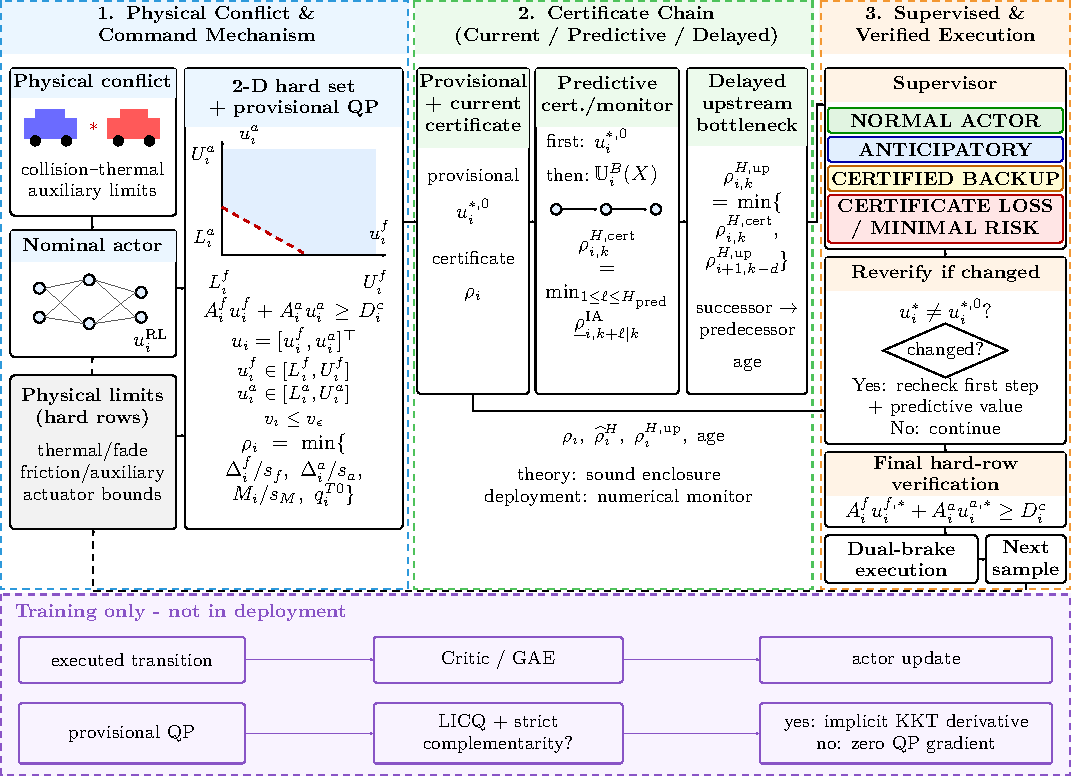
\includegraphics[width=\textwidth]{figures/fig1_desktop66_final.pdf}
\caption{Certificate-aware dual-brake command mechanism. Collision demand and physical limits define the two-dimensional hard set and instantaneous reserve. The theoretical predictive certificate $\rho_{i,k}^{H,{\rm cert}}$ requires sound enclosure; deployment uses the numerical monitor $\widehat{\rho}_{i,k}^{H}$, whose negative value is a warning only. The displayed upstream recursion is theoretical; deployment aggregates age-delayed numerical values for four-mode supervision. A changed action is reverified, and all hard rows are checked before execution. The lower strip denotes training-only secondary diagnostics.}
\label{fig:framework}
\end{figure*}

\section{Related Work}
\subsection{Heavy-Duty Braking and Thermal Fade}
Brake-temperature modeling \cite{talati2009brake}, platoon fade compensation \cite{devika2022fade}, and downhill brake allocation \cite{li2025retarder} motivate the plant but do not test joint collision--thermal feasibility with lagged, gear/power-limited auxiliary actuation.

\subsection{Safety-Constrained Vehicle Control}
CBF-QPs and high-order CBFs (HOCBFs) impose invariance conditions \cite{ames2017cbf,xiao2022hocbf}. Generic exact feasibility \cite{sah2026exact} and reachable-set vehicle model predictive control (MPC) \cite{guo2025uncertainty} do not resolve the coupled thermal dual-brake geometry.

\subsection{Cooperative Platoons and V2V Delay}
Connected controllers use predecessor/leader data for tracking \cite{naus2010string,ploeg2011cacc}; collision invariance and string stability differ. Connected-vehicle CBFs and event-triggered safe reinforcement learning (RL) address networked/intersample uncertainty \cite{li2025connectedcbf,hu2025event}. Zhou \emph{et al.} combine multi-agent RL (MARL), cooperative CBFs, prediction, and a differentiable QP \cite{zhou2026cooperative}; Ohnemus \emph{et al.} study distributed predictive CBFs \cite{ohnemus2026dpcbf}. Our adapted Zhou comparison is a matched domain-transfer test, not a native-domain ranking.

\subsection{Secondary Learning Tools}
Differentiable filters \cite{ma2022differentiable,xiao2023barriernet,yang2023diffcbf} and multi-agent proximal policy optimization (MAPPO) \cite{yu2022mappo} supply one nominal-controller implementation; QP differentiation remains secondary. The gap is physical \emph{command feasibility} under collision, thermal, actuator, and communication constraints (Table~\ref{tab:positioning}).

\begin{table*}[t]
\caption{Scope relative to closest literature; entries describe explicit focus, not ranking.}
\label{tab:positioning}
\centering\normalsize
\begin{tabular}{@{}>{\raggedright\arraybackslash}p{.16\textwidth}>{\raggedright\arraybackslash}p{.15\textwidth}>{\raggedright\arraybackslash}p{.17\textwidth}>{\raggedright\arraybackslash}p{.14\textwidth}>{\raggedright\arraybackslash}p{.11\textwidth}>{\raggedright\arraybackslash}p{.15\textwidth}@{}}
\toprule
Work & Domain & Predictive / reachable & Feasibility / recoverability notion & Diff. QP & Thermal dual brake \\
\midrule
Zhou \emph{et al.} \cite{zhou2026cooperative} & mixed platoon & uncertainty prediction & -- & yes & -- \\
Ohnemus \emph{et al.} \cite{ohnemus2026dpcbf} & modular multi-agent & yes & recoverability & -- & -- \\
Sah--Keshavan \cite{sah2026exact} & multi-robot & -- & yes & -- & -- \\
Guo \emph{et al.} \cite{guo2025uncertainty} & autonomous driving & $n$-step set & -- & -- & -- \\
Hu \emph{et al.} \cite{hu2025event} & automated vehicle & intersample & -- & -- & -- \\
Li \emph{et al.} \cite{li2025retarder} & downhill truck & receding horizon & -- & -- & yes \\
This work & heavy platoon & conditional interval tube & complete instantaneous $\rho$ & local / conditional & yes \\
\bottomrule
\end{tabular}
\end{table*}

\section{Problem Formulation}
Consider a leader indexed by $0$ and $N$ controlled trucks $i\in\{1,\ldots,N\}$ on a road coordinate. Each truck has physical state and brake commands
\begin{equation}
x_i=[p_i,v_i,b_i,r_i,T_i]^\top,\qquad
u_i=[u_i^f,u_i^a]^\top,
\end{equation}
where $p_i,v_i$ are longitudinal position and speed, $b_i,r_i$ are \emph{realized} friction and auxiliary forces, $T_i$ is friction-brake temperature, and $u_i^f,u_i^a$ are their distinct \emph{commands}. The hard QP therefore has exactly two command coordinates. Vehicle $i$ has parameter vector
\begin{equation}
\vartheta_i=(m_i,L_i,c_{r,i},C_{d,i}A_i,\tau_i^f,\tau_i^a,C_i,k_i,\eta_i,\bar b_i),
\end{equation}
where $m_i,L_i,c_{r,i},C_{d,i}A_i$ denote mass, length, rolling resistance, and drag area; $\tau_i^f,\tau_i^a$ are actuator time constants; and $C_i,k_i,\eta_i,\bar b_i$ denote lumped thermal capacity, cooling, friction heating, and cold friction-force capability. Tables~\ref{tab:parameters} and~\ref{tab:nomenclature} summarize provenance and notation.
Hard feasibility is not a function of $x_i$ alone because command memory under zero-order hold, gear availability, dwell logic, and communication validity depend on memory. At sample $k$ the controller therefore uses the augmented hybrid state
\begin{equation}\label{eq:chi}
\begin{aligned}
\chi_{i,k}=[&p_{i,k},v_{i,k},b_{i,k},r_{i,k},T_{i,k},
u^f_{i,k-1},u^a_{i,k-1},g_{i,k},\\
&\tau^g_{i,k},a^{\rm msg}_{i,k},d_{i,k},
v_{i-1,k},a_{i-1,k}]^\top .
\end{aligned}
\end{equation}
Here $g_{i,k}$ is the discrete gear state, $\tau^g_{i,k}$ is the elapsed dwell time in that gear state, $a^{\rm msg}_{i,k}$ is the age of the most recently accepted safety message, $d_{i,k}$ is the inter-vehicle bumper gap, and $v_{i-1,k}$ and $a_{i-1,k}$ are predecessor speed and acceleration. The last three quantities are required by the collision row and predecessor reachable tube. Every certificate below is consequently written as a function of $\chi_{i,k}$, not merely $x_i$.

The time-varying directed vehicle-to-vehicle (V2V) communication graph is $\mathcal G_t=(\mathcal V,\mathcal E_t)$. Agent $i$ observes
\begin{equation}
o_i=(v_i,b_i,r_i,T_i,u^f_{i,k-1},u^a_{i,k-1},g_i,\tau_i^g,
\vartheta_i,\hat\theta_i,d_i,\Delta v_i,
\mathcal M_i),
\end{equation}
where $d_i=p_{i-1}-p_i-L_{i-1}$, $\Delta v_i=v_{i-1}-v_i$, $\hat\theta_i$ is the locally estimated road grade, and $\mathcal M_i$ contains time-stamped permitted messages including the age needed for \eqref{eq:chi}. A message generated at $t_g$ and received at $t$ is replaced by a reachable tube $\mathcal R_{i-1}(t-t_g)$ formed from declared acceleration and jerk bounds. Packets inconsistent with local range/range-rate sensing are rejected, and the union of sensing and communication uncertainty is used in the robust margin. The critic uses global state only during training.

The policy must minimize tracking, comfort, braking-energy, coordination, and intervention costs while maintaining collision, temperature, fade, and actuator constraints. Jerk is a soft comfort constraint and therefore never determines the hard safety feasibility claim. Training, identification, validation, and held-out/out-of-distribution (OOD) test sets are disjoint.

At the transport level, a mission contains a descent profile $\theta(p)$, desired speed schedule, fleet order, payloads, ambient condition, and communication trace. We report
\begin{equation}
J_{\rm op}=\left[t_{\rm trip},E_{\rm fric},E_{\rm aux},e_v^{\rm rms},
e_d^{\rm rms},j^{\rm rms},n_{\rm stop}\right],
\end{equation}
where $E_{\rm fric}=\sum_i\int b_iv_i\,dt$ and $E_{\rm aux}=\sum_i\int r_iv_i\,dt$; $e_v^{\rm rms}$, $e_d^{\rm rms}$, and $j^{\rm rms}$ are speed-error, spacing-error, and jerk root-mean-square (RMS) quantities. Safety is reported separately from efficiency so that an unnecessarily slow method cannot appear superior merely because it avoids demanding maneuvers.

String stability is also separate from safety. With spacing error $e_i^d$, the empirical gains are
\begin{equation}
G_{2,i}=\frac{\|e_i^d\|_2}{\|e_{i-1}^d\|_2+\epsilon_g},\qquad
G_{\infty,i}=\frac{\|e_i^d\|_\infty}{\|e_{i-1}^d\|_\infty+\epsilon_g}.
\end{equation}
Here $\epsilon_g>0$ is a small denominator regularizer that prevents division by zero or a near-zero predecessor-error norm; it is not a safety parameter. We test whether $\max_iG_{2,i}\le1$ and $\max_iG_{\infty,i}\le1$ across platoon lengths; no analytical string-stability theorem is claimed.

\begin{table}[t]
\caption{Vehicle Parameters Required Per Class}
\label{tab:parameters}
\centering\normalsize
\begin{tabular}{@{}>{\raggedright\arraybackslash}p{0.22\columnwidth}>{\raggedright\arraybackslash}p{0.36\columnwidth}>{\raggedright\arraybackslash}p{0.24\columnwidth}@{}}
\toprule
Group & Parameters & Evidence \\
\midrule
Geometry & $m_i,L_i$, axle/load state & weighed vehicle or configuration \\
Resistance & $c_{r,i},C_{d,i}A_i$ & coast-down or source data \\
Actuator & $\tau_i^f,\tau_i^a,\bar u_i^f,\bar u_i^a(v,g)$ & friction and retarder step and power maps \\
Thermal & $C_i,k_i,\eta_i,T_{\rm crit,i}$ & dynamometer or descent fit \\
Fade & $\phi_i(T)$ and uncertainty & held-out force--temperature curve \\
Derivatives & $\dot\theta,\dot q^w,\dot F^r$, predecessor jerk bounds & held-out extrema or certified limits \\
Safety & $a_i^S,t_{h,i},d_{0,i}$ & validated lower bound/policy \\
\bottomrule
\end{tabular}
\end{table}

\begin{table}[t]
\caption{Core Symbols (SI Units Unless Stated)}
\label{tab:nomenclature}
\centering\normalsize
\begin{tabular}{@{}>{\raggedright\arraybackslash}p{0.31\columnwidth}>{\raggedright\arraybackslash}p{0.53\columnwidth}@{}}
\toprule
Symbol & Meaning \\
\midrule
$b,r$ & realized friction and auxiliary brake forces (N) \\
$u^f,u^a$ & commanded friction and auxiliary forces (N) \\
$T,T_a,T_{\rm crit}$ & brake, ambient, and critical temperatures (K) \\
$h^c,h^T,h^F,h^A$ & collision, thermal, fade, and auxiliary barriers \\
$A^f,A^a,D^c$ & collision-row coefficients and demand \\
$[L^f,U^f],[L^a,U^a]$ & effective command intervals after all individual rows \\
$M$ & exact conflict reserve in collision-row units \\
$g^{T0}$ & undivided low-speed state-only thermal reserve (K) \\
$\gamma,\mu$ & directional model and sampled-data margins \\
$H_{\rm QP}$ & safety-QP Hessian; $N_{\rm rec}$ is recovery count \\
\bottomrule
\end{tabular}
\end{table}


Figure~\ref{fig:coupled} summarizes the coupling among friction and auxiliary commands, their actuator lags, longitudinal dynamics, friction heating, and temperature-dependent fade.
\begin{figure*}[t]
\centering
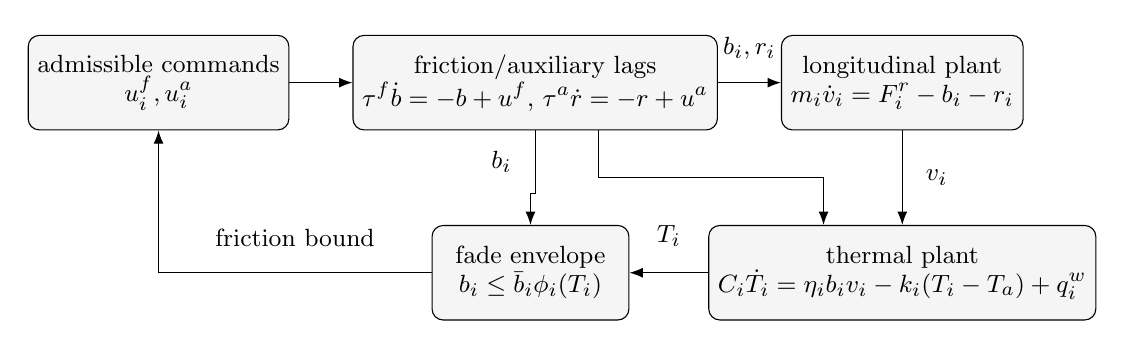
\begin{tikzpicture}[font=\fontsize{9.4}{10.4}\selectfont,>=Latex,node distance=8mm,
 box/.style={draw,rounded corners,minimum width=25mm,minimum height=12mm,align=center,fill=gray!8}]
\node[box] (cmd) {admissible commands\\$u_i^f,u_i^a$};
\node[box,right=of cmd] (lag) {friction/auxiliary lags\\$\tau^f\dot b=-b+u^f$, $\tau^a\dot r=-r+u^a$};
\node[box,right=of lag] (long) {longitudinal plant\\$m_i\dot v_i=F_i^r-b_i-r_i$};
\node[box,below=12mm of long] (heat) {thermal plant\\$C_i\dot T_i=\eta_i b_i v_i-k_i(T_i-T_a)+q_i^w$};
\node[box,left=10mm of heat] (fade) {fade envelope\\$b_i\le \bar b_i\phi_i(T_i)$};
\draw[->] (cmd)--(lag);
\draw[->] (lag)--node[midway,above=5pt]{$b_i,r_i$}(long);
\draw[->] (lag.south) -- node[midway,left=5pt]{$b_i$} ++(0,-8mm) -| (fade.north);
\draw[->] ([xshift=8mm]lag.south) -- ++(0,-6mm) -| ([xshift=-10mm]heat.north);
\draw[->] (long)--node[midway,right=5pt]{$v_i$}(heat);
\draw[->] (heat)--node[midway,above=6pt]{$T_i$}(fade);
\draw[->] (fade.west) -- node[midway,above=6pt]{friction bound} (cmd.south |- fade.west) -- (cmd.south);
\end{tikzpicture}

\caption{Coupling among friction and auxiliary commands, their distinct actuator lags, longitudinal motion, friction heating, and the temperature-dependent fade envelope.}
\label{fig:coupled}
\end{figure*}

\section{Heavy-Duty Dual-Brake Dynamics and Physical Constraints}
\subsection{Dual-Brake Longitudinal--Thermal Model}
With positive road angle uphill, define the nonbraking force
\begin{equation}
F_i^r=F_i^d-m_ig\sin\theta_i-m_igc_{r,i}\cos\theta_i-
\tfrac12\rho_{\rm air}C_{d,i}A_iv_i^2+w_i,
\end{equation}
where $\rho_{\rm air}$ is air density, $F_i^d$ is the modeled driveline-force contribution, and $w_i$ is the lumped residual longitudinal force/disturbance term. The model is
\begin{subequations}\label{eq:model}
\begin{align}
\dot p_i&=v_i, & m_i\dot v_i&=F_i^r-b_i-r_i,\\
\tau_i^f\dot b_i&=-b_i+u_i^f,
&\tau_i^a\dot r_i&=-r_i+u_i^a,\\
C_i\dot T_i&=\eta_i b_iv_i-k_i(T_i-T_a)+q_i^w.
\end{align}
\end{subequations}
The auxiliary envelope captures retarder/engine-brake power, shaft-speed, gear, and response restrictions:
\begin{equation}\label{eq:auxenv}
0\le r_i\le\bar r_i(v_i,g_i),\quad
0\le u_i^a\le\bar u_i^a(v_i,g_i).
\end{equation}
Each command is constant on the open zero-order-hold (ZOH) interval and may change at a sample instant. No independent physical command-slew limit is asserted. The realized forces remain continuous through the identified first-order actuator dynamics in \eqref{eq:model}.
Realized-force availability is not implied by the command envelope. Define the longitudinal acceleration $a_i:=\dot v_i$. For a fixed valid gear branch during one ZOH interval, define $h_i^A=\bar r_i(v_i,g_i)-r_i$ and $\bar r_{i,v}:=\partial\bar r_i(v_i,g_i)/\partial v_i$. Its robust CBF gives
\begin{equation}\label{eq:auxcbf}
u_i^a\le r_i+\tau_i^a\!\left[\bar r_{i,v}a_i+\alpha_A(h_i^A)-\gamma_i^A-\mu_i^A\right].
\end{equation}
For permitted shifts, the controller uses the minimum valid envelope over reachable gears and enforces the manufacturer's dwell time; no derivative is taken through a gear discontinuity.
The friction envelope is $0\le b_i\le\bar b_i\phi_i(T_i)$, where $\phi_i'(T)\le0$ on a calibrated interval. Parameters and residual/derivative bounds must be identified on separate data.

The selected functions $\alpha_{1c},\alpha_{2c},\alpha_{1T},\alpha_{2T},\alpha_F$, and $\alpha_A$ are locally Lipschitz extended class-$\mathcal K$ functions on the declared operating domain. Their choices are fixed before evaluation; no gain is inferred from the reported outcomes.

\subsection{Collision HOCBF}
Let $a_i^S>0$ lower-bound follower braking, $a_{i-1}^E>0$ upper-bound predecessor emergency deceleration, and $t_{h,i},d_{0,i}$ denote prescribed time headway and standstill spacing. With $q_i=t_{h,i}+\tau_i^f$,
\begin{equation}\label{eq:hc}
h_i^c=d_i-d_{0,i}-q_iv_i-\frac{v_i^2}{2a_i^S}
+\frac{v_{i-1}^2}{2a_{i-1}^E}.
\end{equation}
Set $c_i=q_i+v_i/a_i^S$ and $r_{i-1}^v=v_{i-1}/a_{i-1}^E$. Then
\begin{align}
\dot h_i^c&=v_{i-1}-v_i-c_ia_i+r_{i-1}^va_{i-1},\label{eq:hcdot}\\
\ddot h_i^c&=a_{i-1}-a_i-\frac{a_i^2}{a_i^S}-c_i\dot a_i
+\frac{a_{i-1}^2}{a_{i-1}^E}+r_{i-1}^v\dot a_{i-1}.\label{eq:hcddot}
\end{align}
The continuous-time jerk is
\begin{equation}\label{eq:jerk}
j_i=\dot a_i=\frac{\dot F_i^r}{m_i}+\frac{b_i-u_i^f}{m_i\tau_i^f}
+\frac{r_i-u_i^a}{m_i\tau_i^a}.
\end{equation}
Hence both commands enter $\ddot h_i^c$ with positive coefficients. For $\psi_{1i}^c=\dot h_i^c+\alpha_{1c}(h_i^c)$, the sampled-data-tightened robust HOCBF is
\begin{equation}\label{eq:collision_hocbf}
A_i^fu_i^f+A_i^au_i^a+\widehat\Xi_i^c-\gamma_i^c-\mu_i^c
+\alpha_{2c}(\psi_{1i}^c)\ge0,
\end{equation}
where $A_i^f=c_i/(m_i\tau_i^f)>0$, $A_i^a=c_i/(m_i\tau_i^a)>0$, and $\mu_i^c$ is the intersample tightening.

\subsection{Temperature HOCBF and Fade CBF}
Let $h_i^T=T_{\rm crit,i}-T_i$. Its first derivative contains no command. Differentiation gives
\begin{equation}
\ddot h_i^T=-\frac{\eta_iv_i}{C_i\tau_i^f}u_i^f+\Xi_i^T,
\end{equation}
where, for constant thermal parameters,
\begin{equation}
\widehat\Xi_i^T=\frac{\eta_ib_iv_i}{C_i\tau_i^f}-\frac{\eta_ib_ia_i}{C_i}
+\frac{k_i}{C_i}(\dot T_i-\dot T_a)-\frac{\widehat{\dot q_i^w}}{C_i}.
\end{equation}
Rather than differentiating noisy heat residuals, implementation bounds $\dot q_i^w$, $\dot T_a$, grade rate, and resistance derivatives. With $\psi_{1i}^T=\dot h_i^T+\alpha_{1T}(h_i^T)$,
\begin{equation}\label{eq:thermal_hocbf}
-B_i^fu_i^f+\widehat\Xi_i^T-\gamma_i^T-\mu_i^T
+\alpha_{2T}(\psi_{1i}^T)\ge0,
\quad B_i^f=\frac{\eta_iv_i}{C_i\tau_i^f}.
\end{equation}
Temperature therefore caps friction braking but does not directly cap auxiliary braking.

The fade envelope is enforced dynamically rather than checked as a state-only row. Define
\begin{equation}
h_i^F=\bar b_i\phi_i(T_i)-b_i.
\end{equation}
The first-order robust CBF $\dot h_i^F+\alpha_F(h_i^F)\ge0$ yields the explicit upper bound
\begin{equation}\label{eq:fade_cbf}
u_i^f\le b_i+\tau_i^f\!\left[\bar b_i\phi_i'(T_i)\dot T_i
+\alpha_F(h_i^F)-\gamma_i^F-\mu_i^F\right].
\end{equation}
Let $v_\epsilon$ denote the specified low-speed switching threshold. At $v_i\le v_\epsilon$, $B_i^f$ is too small for a meaningful division. Under ZOH commands and constant $v_i,T_a,q_i^w$ over $[t_k,t_k+\Delta t]$, set $\lambda_i=k_i/C_i$, $E_i=e^{-\lambda_i\Delta t}$,
\begin{equation}
I_{0i}=\frac{1-E_i}{\lambda_i},\qquad
I_{1i}=E_i\frac{e^{(\lambda_i-1/\tau_i^f)\Delta t}-1}{\lambda_i-1/\tau_i^f},
\end{equation}
using the continuous limits when a denominator vanishes. Exact integration yields
\begin{align}
T_{i,k+1}={}&T_a+E_i(T_{i,k}-T_a)+\frac{q_i^wI_{0i}}{C_i}\nonumber\\
&+\frac{\eta_i v_i}{C_i}\{b_{i,k}I_{1i}+u_{i,k}^f(I_{0i}-I_{1i})\}.\label{eq:zohthermal}
\end{align}
Separate the command-independent prediction
\begin{equation}
T_{i,k+1}^{\rm base}=T_a+E_i(T_{i,k}-T_a)+q_i^wI_{0i}/C_i+\eta_i v_i b_{i,k}I_{1i}/C_i
\end{equation}
and define the undivided state-side thermal reserve
\begin{equation}\label{eq:gT0}
g_{i,k}^{T0}=T_{\rm crit,i}-\Delta_T-\bar e_i^T-T_{i,k+1}^{\rm base}.
\end{equation}
Here $\Delta_T>0$ is the registered temperature safety buffer below $T_{\rm crit,i}$ used by the low-speed one-step thermal constraint.
The low-speed hard row is $c_i^Tu_{i,k}^f\le g_{i,k}^{T0}$, where $c_i^T=\eta_iv_i(I_{0i}-I_{1i})/C_i$. It is retained without division. At $v_i=0$, $c_i^T=0$ exactly and the row becomes the command-independent condition $0\le g_{i,k}^{T0}$; therefore $g_{i,k}^{T0}<0$ is hard infeasibility even if both command intervals and the collision row remain feasible. The term $\bar e_i^T$ is computed by \eqref{eq:zoherror} from registered bounds on $|a|$, $|\dot T_a|$, $|\dot q^w|$, thermal parameters, friction lag, and integration error.

\subsection{Directional Robust and Digital Margins}
Define $\zeta_i$ as the collection of measured local/predecessor states, predecessor acceleration and jerk, message age, packet delay, grade and grade rate, rolling and aerodynamic forces, $q_i^w$ and $\dot q_i^w$, and both actuator lags. The box $\mathcal B_i(\hat\zeta_i)=\prod_j[\hat\zeta_{ij}-\varepsilon_{ij}^-,\hat\zeta_{ij}+\varepsilon_{ij}^+]$ includes sensor error and identified parameter/residual intervals. Packet loss acts through message age and a predecessor reachable tube; if age exceeds its registered horizon, the bound is invalid and the supervisor triggers. If $\widehat\Xi_i^k$ is the computed uncontrolled term and $\Xi_i^k$ is the true term, the correct one-sided margin is
\begin{equation}\label{eq:margin}
\gamma_i^k\ge\sup_{\zeta\in\mathcal B_i(\hat\zeta_i)}
\{\widehat\Xi_i^k-\Xi_i^k(\zeta)\},\quad k\in\{c,T,F,A\}.
\end{equation}
Thus $\widehat\Xi_i^k-\gamma_i^k\le\Xi_i^k$; an absolute-error bound is sufficient but unnecessarily conservative. In the theoretical construction, a sound interval arithmetic (IA) lower endpoint $\underline\Xi_i^k$ gives $\gamma_i^k=\max\{0,\widehat\Xi_i^k-\underline\Xi_i^k\}$. The present floating-point implementation has no verified directed-rounding enclosure. Measurement intervals cover position, speed, acceleration, and brake-state sensing; dynamics intervals cover grade/grade rate, resistance, aerodynamics, heat residual/rate, and lag uncertainty; communication intervals cover age/delay plus reachable acceleration/jerk. Each digital rate bound $L_i^k$ is computed by the executable product-rule expression \eqref{eq:ratebound}, and $\mu_i^k=L_i^k\Delta t+\bar e_{\rm int,i}^k$. Empirical quantiles are not used as deterministic bounds.

\section{Certificate-Aware Dual-Brake Control}
\subsection{Hard Safety Polytope and Viability Reserve}
The canonical forward decision is exactly $u_i=[u_i^f,u_i^a]^\top\in\mathbb R^2$. Jerk is evaluated as a comfort metric after the action is applied; it is neither a QP coordinate nor a slack variable. The hard projection is
\begin{subequations}\label{eq:qp}
\begin{align}
u_i^*=\arg\min_{u_i\in\mathbb R^2}\;&\tfrac12(u_i-u_i^{\rm RL})^\top W_i(u_i-u_i^{\rm RL})
+\epsilon\|u_i\|^2\\
\mathrm{s.t.}\;&\eqref{eq:collision_hocbf},\ \eqref{eq:thermal_hocbf},\ \eqref{eq:fade_cbf},\ \eqref{eq:auxcbf},\\
&0\le u_i^f\le\bar u_i^f,\quad 0\le u_i^a\le\bar u_i^a(v_i,g_i),\\
&c_i^Tu_i^f\le g_{i,k}^{T0}\ \text{when }v_i\le v_\epsilon.
\end{align}
\end{subequations}
Here $u_i^{\rm RL}$ is the nominal preprojection command supplied by the policy used in this implementation; the certificate and hard QP accept any nominal command in the declared bounds. $W_i\succeq0$ is the command weighting and $\epsilon>0$ the regularizer, so $H_{{\rm QP},i}=W_i+2\epsilon I\succ0$. No hard row has slack in certified operation.

For $v_i>v_\epsilon$, the thermal HOCBF contributes to the friction interval; for $v_i\le v_\epsilon$, it is replaced, not supplemented, by the undivided ZOH row. All command-dependent noncollision rows reduce to individual intervals $u_i^f\in[L_i^f,U_i^f]$ and $u_i^a\in[L_i^a,U_i^a]$: the friction interval intersects command magnitude, active thermal-mode, and fade bounds; the auxiliary interval intersects command magnitude, gear/power, and realized-force-CBF bounds. For $0<v_i\le v_\epsilon$, $c_i^T>0$ and the ZOH row is absorbed by $U_i^f=\min\{U_i^{f,\mathrm{other}},g_{i,k}^{T0}/c_i^T\}$; at $v_i=0$ it is the state-only gate $g_{i,k}^{T0}\ge0$. The collision row is the sole command-coupled face,
\begin{equation}\label{eq:collisiondemand}
A_i^fu_i^f+A_i^au_i^a\ge D_i^c,\quad
D_i^c=\gamma_i^c+\mu_i^c-\widehat\Xi_i^c-\alpha_{2c}(\psi_{1i}^c).
\end{equation}
The physical collision-demand reserve is
\begin{equation}\label{eq:reserve}
M_i(\chi_{i,k})=A_i^fU_i^f+A_i^aU_i^a-D_i^c.
\end{equation}
It remains interpretable if an individual interval is empty, but its sign alone is then insufficient. Define $\Delta_i^f=U_i^f-L_i^f$, $\Delta_i^a=U_i^a-L_i^a$, and
\begin{equation}
q_{i,k}^{T0}=\begin{cases}g_{i,k}^{T0}/s_{T0},&v_i\le v_\epsilon,\\+\infty,&v_i>v_\epsilon,\end{cases}
\end{equation}
where $s_{T0}>0$ is a fixed temperature scale. With fixed positive normalizers $s_f$ [N], $s_a$ [N], and $s_M$ [m/s$^2$], define the complete signed certificate
\begin{equation}\label{eq:rho}
\rho_i(\chi_{i,k})=\min\!\left\{\Delta_i^f/s_f,\Delta_i^a/s_a,M_i(\chi_{i,k})/s_M,q_{i,k}^{T0}\right\}.
\end{equation}
We fix $s_f$ to reference cold friction-force capability, $s_a$ to reference auxiliary-force capability, $s_M$ to a reference deceleration/barrier-row scale, and $s_{T0}$ to a fixed one-step temperature scale. They are shared by every algorithm and never retuned per method. Positive choices preserve the sign but affect magnitude, trigger time, learning loss, and the normalized critical component; therefore $\Delta_i^f$, $\Delta_i^a$, $M_i$, and low-speed $g_{i,k}^{T0}$ are always logged and evaluated in a fixed scale-sensitivity study. Instantaneous feasibility is
\begin{equation}\label{eq:instantfeas}
\mathsf{Feas}_{i,k}:=(\rho_i(\chi_{i,k})\ge0).
\end{equation}
Thus nonnegative $M_i$ never hides an empty interval or a failed zero-coefficient thermal row: $M_i$ remains the physical collision supply-minus-demand term, while $\rho_i$ is the complete exact certificate. For fixed auxiliary command,
\begin{align}
u_i^f&\ge\ell_i^c(u_i^a)=\frac{D_i^c-A_i^au_i^a}{A_i^f},\label{eq:lower}\\
u_i^f&\le U_i^f.\label{eq:upper}
\end{align}
The exact minimum in \eqref{eq:rho} is used for certification; only the learning path may smooth it.

\subsection{Predictive Feasibility Formulation and Distributed Bottleneck Monitoring}
Let $H_{\rm pred}$ be the theoretical predictive horizon in samples and $\mathcal X^B_{i,k\mid k}=\{\chi_{i,k}\}$. At step $\ell$, let $\Omega_\ell$ be the declared uncertainty box and $\mathbb U_i^B(\mathcal X)$ a sound set-valued command enclosure of the pointwise backup law $\kappa_i^B$, so $\{\kappa_i^B(\chi):\chi\in\mathcal X\}\subseteq\mathbb U_i^B(\mathcal X)$. Under the sound-enclosure assumption, the closed-loop tube obeys
\begin{equation}\label{eq:tube}
\mathcal X^B_{\ell+1}\supseteq\mathcal F_i^{\rm IA}(\mathcal X^B_\ell,\mathbb U_i^B(\mathcal X^B_\ell),\Omega_\ell).
\end{equation}
Table~\ref{tab:predictive_symbols} summarizes the predictive and learning notation, including the learning horizon $H_L$ in samples. Table~\ref{tab:constraints} distinguishes the hard projection rows from quantities, such as jerk, that lie outside the hard QP.
The theoretical $\mathcal F_i^{\rm IA}$ must soundly enclose the sampled plant and all admissible discrete branches; $\Omega_\ell$ covers plant, predecessor, thermal, gear, and communication uncertainty. The first transition uses provisional $u_{i,k}^{*,0}$; for $\ell\ge2$, $\mathbb U_i^B(\mathcal X)$ must outwardly enclose every pointwise backup command. A center-point trajectory is not certified. The evaluated fixed-gear, affine-saturation implementation uses native floating-point endpoints without directed rounding, complete gear/dwell branch hulls, or a global reserve-enclosure proof. Its predictive output is thus a numerical warning monitor; backup interval widths are logged.

For comparison define the generally intractable true robust reserve
\begin{equation}
\rho_{i,k}^{H,{\rm true}}=\min_{1\le\ell\le H_{\rm pred}}\inf_{\chi\in\mathcal X^B_{i,k+\ell\mid k}}\rho_i(\chi).
\end{equation}
Under sound enclosure, the interval evaluation supplies a lower bound,
\begin{align}
\underline\rho^{\rm IA}_{i,k+\ell\mid k}
&\le\inf_{\chi\in\mathcal X^B_{i,k+\ell\mid k}}\rho_i(\chi),\label{eq:predlower}\\
\rho_{i,k}^{H,{\rm cert}}
&=\min_{1\le\ell\le H_{\rm pred}}\underline\rho^{\rm IA}_{i,k+\ell\mid k}.\label{eq:rhocert}
\end{align}
Under sound enclosure, $\rho^{H,{\rm cert}}\ge0$ certifies robust hard feasibility; a negative value is inconclusive without exact reachable-set optimization. The unverified numerical monitor records the minimizing step and physical row.
The evaluated floating-point implementation returns the numerical counterpart $\widehat{\rho}_{i,k}^{H}$; unlike $\rho_{i,k}^{H,{\rm cert}}$, it is not claimed to be a formally sound enclosure. Its sign is a monitoring signal, not a proof of future feasibility or infeasibility.

For the theoretical certificate, the centralized minimum is
\begin{equation}\label{eq:fleetreserve}
\rho_{{\rm fleet},k}^{H,{\rm cert}}=\min_i\rho_{i,k}^{H,{\rm cert}},
\end{equation}
and is used only by centralized training/evaluation. Deployment uses successor-to-predecessor recursive aggregation
\begin{align}
\rho_{i,k}^{H,{\rm up}}&=\min\{\rho_{i,k}^{H,{\rm cert}},\rho_{i+1,k-d}^{H,{\rm up}}\},\label{eq:minconsensus}\\
m_{i,k}^{\rm safe}&=(\rho_{i,k}^{H,{\rm up}},i_{\rm crit},\ell_{\rm crit},q_{\rm crit},t_k),
\end{align}
Here $d$ is accepted message age in samples; $i_{\rm crit}$, $\ell_{\rm crit}$, and $q_{\rm crit}$ identify the limiting vehicle, step, and physical row. Missing or over-age messages invoke a conservative age bound. Each truck thus knows only an age-bounded local/upstream aggregate, not the instantaneous global minimum.
Equation~\eqref{eq:minconsensus} states the theoretical recursion. The deployed recursion uses $\widehat{\rho}_{i,k}^{H}$ as its local operand and age-delayed numerical messages; neither its value nor its attribution is an instantaneous fleet-global certificate.

\begin{table}[t]
\caption{Predictive and learning symbols.}
\label{tab:predictive_symbols}
\centering\normalsize
\begin{tabular}{@{}>{\raggedright\arraybackslash}p{0.34\columnwidth}>{\raggedright\arraybackslash}p{0.52\columnwidth}@{}}
\toprule
Symbol & Definition \\
\midrule
$H_{\rm pred}$ & theoretical predictive horizon (samples) \\
$H_L$ & differentiable learning horizon (samples) \\
$\tau_s>0$ & learning soft-min temperature \\
$\mathcal F^{\rm IA}$ & theoretical sound interval set map \\
$\rho_{i,k}^{H,{\rm cert}}$ & theoretical one-sided certificate under sound enclosure \\
$\widehat{\rho}_{i,k}^{H}$ & evaluated floating-point predictive monitor \\
$\Omega_\ell$ & declared uncertainty box at step $\ell$ \\
$\kappa^B,\mathbb U^B$ & point backup and command-set extension \\
$\epsilon_{\rm th},\epsilon_\tau$ & thermal-parameter and lag relative bounds \\
$s_f,s_a,s_M,s_{T0}$ & fixed physical certificate normalizers \\
$\rho_{\rm pred,trig},\rho_{\rm hard,trig}$ & predictive and hard trigger levels \\
$\rho_{\rm pred,rec},\rho_{\rm hard,rec}$ & hysteretic recovery levels \\
$N_{\rm rec}$ & consecutive recovery samples \\
\bottomrule
\end{tabular}
\end{table}


\begin{table}[t]
\caption{Projection Constraints and Guarantee Status}
\label{tab:constraints}
\centering\normalsize
\begin{tabular}{@{}>{\raggedright\arraybackslash}p{0.25\columnwidth}>{\raggedright\arraybackslash}p{0.13\columnwidth}>{\raggedright\arraybackslash}p{0.43\columnwidth}@{}}
\toprule
Constraint & Default & Consequence of relaxation \\
\midrule
Spacing HOCBF & hard & positive slack removes strict collision claim \\
Thermal HOCBF & hard & positive slack removes thermal invariance claim \\
Fade CBF & hard & positive slack removes fade-envelope invariance \\
Friction and auxiliary envelopes & hard & relaxation can request unavailable force/power \\
Auxiliary envelope and realized-force CBF & hard & relaxation can violate lag/gear availability \\
Low-speed ZOH thermal row & hard & relaxation removes the near-stop thermal claim \\
Jerk & outside QP & comfort metric; not part of hard feasibility \\
Tracking objective & soft & performance degradation only \\
\bottomrule
\end{tabular}
\end{table}


\subsection{Secondary Learning Diagnostic}
Under CTDE, the shared actor samples $\epsilon_i\sim\mathcal N(0,I)$, sets $y_i=\mu_\theta(o_i)+\sigma_\theta(o_i)\odot\epsilon_i$, and maps to physical nominal bounds by $u_{ij}^{\rm RL}=l_{ij}+(h_{ij}-l_{ij})(\tanh y_{ij}+1)/2$. Its nominal log density includes Gaussian and $\tanh$/affine Jacobian terms. Proximal policy optimization (PPO) ratios use the nominal sample; the centralized critic and generalized advantage estimation (GAE) use the executed $u_i^*$ and transition.

The paired diagnostic augments the usual clipped PPO objective with an intervention term
\begin{equation}\label{eq:actorloss}
\mathcal J_\theta=\mathcal L_{\rm clip}+\beta\mathcal H(\pi_\theta)
-\lambda_I\mathbb E\|u_i^{*,0}-u_i^{\rm RL}\|_{W_i}^{2}.
\end{equation}
Here $\beta,\lambda_I\ge0$ weight entropy and fixed intervention penalty. Matched branches share nominal sample, reward, two-dimensional forward QP, execution, critic target, and optimizer. DiffQP differentiates provisional $u_i^{*,0}$ only when regularity gates pass; StopGradient detaches that output path, retaining direct dependence on $u_i^{\rm RL}$. Interval extrema, supervisor, messages, backup switches, and plant remain stop-gradient; rewards never replace hard rows.

\subsection{Karush--Kuhn--Tucker (KKT) Differentiation}
Write the strongly convex two-variable QP as $\min_u u^\top H_{\rm QP}u/2-(Bp+h)^\top u$ subject to $Gu\le q$. In forward projection, $p=u^{\rm RL}$, $H_{\rm QP}=W+2\epsilon I$, $B=W$, and $h=0$; omitted $p^\top Wp/2$ is constant in $u$. For active rows $\mathcal A$ satisfying linear independence constraint qualification (LICQ) and strict complementarity,
\begin{equation}\label{eq:kktdiff}
\begin{bmatrix}H_{\rm QP}&G_{\mathcal A}^\top\\G_{\mathcal A}&0\end{bmatrix}
\begin{bmatrix}\partial u^*/\partial p\\\partial\lambda_{\mathcal A}^*/\partial p\end{bmatrix}
=\begin{bmatrix}B\\0\end{bmatrix}.
\end{equation}
At active-set switches a classical derivative may not exist. In $\mathbb R^2$, over two active inequality gradients cannot satisfy LICQ; four commonly activate in the calibrated learning cases. The forward QP remains valid, but the selected local derivative is unavailable, so a predefined zero-QP-gradient fallback preserves the forward action. Regular-case finite-difference tests check the derivative; Results report the formal learning outcome.

\subsection{Supervisory Backup and Recovery}
Define the backup-feasible domain
\begin{equation}
\begin{split}
\mathcal K_i^B=\{\chi_i:\;&h_i^c,h_i^T,h_i^F,h_i^A,\psi_{1i}^c,\psi_{1i}^T,\rho_i,v_i\ge0,\\
&q_i^{\rm gear/dwell}=1,\ q_i^{\rm comm}=1\},
\end{split}\label{eq:backupdomain}
\end{equation}
where the two Boolean mode indicators mean that gear/dwell logic is admissible and the declared communication uncertainty bound remains valid. The auxiliary state barrier $h_i^A\ge0$ is not implied by the command interval and is therefore explicit. Choose fixed dimensionless thresholds $\rho_{\rm pred,trig}>\rho_{\rm hard,trig}\ge0$ and recovery levels $\rho_{\rm pred,rec}>\rho_{\rm pred,trig}$ and $\rho_{\rm hard,rec}>\rho_{\rm hard,trig}$. The deployed supervisor compares $\widehat{\rho}_{i,k}^{H}$ with predictive thresholds as a warning monitor, not as a formal future-feasibility certificate. It has four modes: (i) NORMAL ACTOR; (ii) ANTICIPATORY when $\widehat{\rho}_{i,k}^{H}\le\rho_{\rm pred,trig}$, applying early auxiliary braking, headway expansion, and an upstream request; (iii) CERTIFIED BACKUP when $\rho_i\le\rho_{\rm hard,trig}$ or a hard residual fails; and (iv) CERTIFICATE LOSS/MINIMAL RISK when $\rho_i<0$. Recovery requires $N_{\rm rec}$ consecutive samples above both recovery levels.

If the backup hard polytope is empty, no controller using the declared actuators can guarantee all constraints. The minimal-risk mode commands maximum feasible auxiliary braking, caps friction at the temperature/fade bound, requests upstream deceleration and headway expansion, and initiates a controlled stop; it records loss of certificate rather than silently using safety slack.

\subsection{Training and Execution Algorithm}
The executable two-pass order is: (1) measure/time-align state and messages; (2) construct robust/digital margins and hard command intervals; (3) obtain a nominal command $u_{i,k}^{\rm RL}$; (4) solve the normal hard QP for provisional $u_{i,k}^{*,0}$; (5) compute instantaneous $\rho_i$ and propagate the numerical predictive tube using $u_{i,k}^{*,0}$ first and $\mathbb U_i^B(\mathcal X)$ thereafter; (6) evaluate $\widehat{\rho}_{i,k}^{H}$, physical attribution, the age-bounded recursive bottleneck, and supervisor mode; (7) keep $u^{*,0}$ in NORMAL, otherwise solve the anticipatory QP or backup; (8) if final $u_i^*\ne u_i^{*,0}$, re-evaluate the first transition and predictive value or run the equivalent fast verifier; (9) validate every final hard-row residual and apply $u_i^*$; and (10) log nominal, provisional, final, and both provisional/final predictive values. The implementation exposes this order as one non-reorderable routine. Deployment removes the critic and privileged centralized minimum.

\section{Safety and Predictive-Feasibility Analysis}
\textbf{Assumption 1 (regular bounded model):} On a compact operating domain, \eqref{eq:model} is locally Lipschitz; masses, lags, and heat capacities are bounded away from zero; directional and digital margins dominate all declared estimation, derivative, communication, integration, and sampled-model errors.

\textbf{Assumption 2 (valid backup tube):} $\Omega_{k:k+H}$ contains the true grade/grade rate, predecessor acceleration/jerk, mass/resistance, actuator lags, thermal/fade error, ambient variation, heat-flow residual, gear/power availability, and message age/delay. The first set transition uses the already computed provisional $u_{i,k}^{*,0}$; later transitions use a sound command-set extension $\mathbb U_i^B(\mathcal X)$ of the state-feedback backup. If the supervisor changes the applied command, the first transition is re-evaluated before application.

\textbf{Proposition 1 (complete instantaneous equivalence):} Under the two individual intervals, the coupled row in \eqref{eq:collisiondemand}, and the active low-speed state gate \eqref{eq:gT0}, the hard command set is nonempty if and only if $\rho_i(\chi_{i,k})\ge0$.

\emph{Proof:} All normalizers are positive. At $v_i>v_\epsilon$, $q_{i,k}^{T0}=+\infty$ and the three command-dependent terms give the result. For $0<v_i\le v_\epsilon$, exact zero-order-hold integration gives $c_i^T=\eta_i v_i(I_{0i}-I_{1i})/C_i>0$. Write $U_i^{f,\mathrm{other}}$ for the upper friction bound before the low-speed thermal row and set
\begin{equation}\label{eq:low-speed-upper}
U_i^{f,\mathrm{LS}}=\min\{U_i^{f,\mathrm{other}},g_{i,k}^{T0}/c_i^T\}.
\end{equation}
The $U_i^f$ used in $\Delta_i^f$ and $M_i$ is this intersection in the low-speed branch. Hence the undivided row is satisfied by every $u_i^f\le U_i^f$; $g_{i,k}^{T0}\ge0$ also remains the explicit state-side gate in the implemented certificate. At $v_i=0$, $c_i^T=0$, division is not performed, and the row is exactly the state-only condition $0\le g_{i,k}^{T0}$. At every speed, the command intervals are nonempty precisely when $\Delta_i^f,\Delta_i^a\ge0$. Since $A_i^f,A_i^a>0$, the collision left side is maximal at $(U_i^f,U_i^a)$ and meets demand precisely when $M_i\ge0$. These conditions are exactly the nonnegative components of $\rho_i$; reversing each step proves necessity.

\textbf{Proposition 2 (one-sided robust certificate):} Under Assumption 2, if $\rho_{i,k}^{H,{\rm cert}}\ge0$, then the hard command set is nonempty at every predicted sample for every declared realization.

\emph{Proof:} Sound set propagation places every closed-loop realization in $\mathcal X^B_{i,k+\ell\mid k}$. By \eqref{eq:predlower}, $\rho_i(\chi_{i,k+\ell})\ge\inf_{\chi\in\mathcal X^B}\rho_i(\chi)\ge\underline\rho^{\rm IA}_{i,k+\ell\mid k}\ge\rho_{i,k}^{H,{\rm cert}}$. Proposition 1 applies. Conversely, $\rho_{i,k}^{H,{\rm cert}}<0$ is inconclusive because dependency inflation can lower the interval evaluation below the true infimum. This establishes neither global nor post-horizon recursive feasibility.

\textbf{Proposition 3 (horizon monotonicity):} For a common stored prefix of IA lower bounds, $\rho_i^{H+1,{\rm cert}}\le\rho_i^{H,{\rm cert}}$.

\emph{Proof:} The longer-horizon minimum contains every old lower bound and one additional term.

\textbf{Proposition 4 (closed-loop uncertainty monotonicity):} Let $\Omega_1\subseteq\Omega_2$. Suppose $\mathcal F^{\rm IA}$ is inclusion monotone in state, command, and uncertainty sets, and $\mathbb U^B$ is an inclusion-monotone set extension of the state-feedback backup. Starting from the same singleton, the resulting tubes are nested and $\rho_i^{H,{\rm cert}}(\Omega_2)\le\rho_i^{H,{\rm cert}}(\Omega_1)$ whenever the IA certificate evaluator is inclusion antitone under set enlargement.

\emph{Proof:} Induction: equal initial sets are nested. If $\mathcal X_{1,\ell}\subseteq\mathcal X_{2,\ell}$, inclusion monotonicity gives $\mathbb U^B(\mathcal X_{1,\ell})\subseteq\mathbb U^B(\mathcal X_{2,\ell})$ and then $\mathcal X_{1,\ell+1}\subseteq\mathcal X_{2,\ell+1}$. Lower interval endpoints cannot increase under the stated antitone evaluator; the horizon minimum preserves order. The executable affine-plus-saturation backup satisfies these properties and is regression-tested. No theorem is asserted for an arbitrary non-monotone custom enclosure.

\textbf{Proposition 5 (centralized and recursive minima):} The centralized $\rho_{{\rm fleet},k}^{H,{\rm cert}}\ge0$ if and only if every truck certificate is nonnegative. With zero-delay complete chain delivery, recursive \eqref{eq:minconsensus} at the head equals that centralized minimum and propagates an attaining argmin. With delay/loss it is instead an age-bounded local/upstream quantity using the registered conservative stale-message replacement.

\emph{Proof:} The centralized statement follows from the finite minimum. Recursive pairwise minima are associative and propagate the chosen metadata. Stale replacement changes the operand, so equality with the instantaneous centralized minimum is not claimed.

\textbf{Corollary (physical sensitivities):} Holding all other limits fixed, increasing $U_i^a$ cannot decrease $M_i$, and increasing either individual upper bound cannot decrease $\rho_i$. If the calibrated fade map and every temperature-dependent friction upper bound are nonincreasing in $T_i$, increasing initial temperature cannot increase $\rho_i$. Nested grade or age uncertainty cannot increase $\rho_i^{H,{\rm cert}}$ only under Proposition 4's inclusion assumptions. No monotonicity is asserted when other state-dependent terms change simultaneously.

\textbf{Proposition 6 (sampled-data preservation):} Let each held-command barrier left-hand side $F_i^q$, $q\in\{c,T,F,A\}$, obey $|\dot F_i^q|\le L_i^q$ and have integration error $\bar e_i^q$. Tightening by $\mu_i^q=L_i^q\Delta t+\bar e_i^q$ preserves the continuous row between samples. The executable product-rule bound is
\begin{equation}\label{eq:ratebound}
L_i^q=\bar\xi_{q,\dot{}}+\sum_j(\bar a_{qj}\bar{\dot u}_j+\bar{\dot a}_{qj}\bar u_j),
\end{equation}
with separately registered component bounds for collision, thermal, fade, and auxiliary rows. During each open ZOH interval, $\dot u_j=0$, so the implemented held-command specialization is $L_i^q=\bar\xi_{q,\dot{}}+\sum_j\bar{\dot a}_{qj}\bar u_j$; command jumps are evaluated anew at sample instants.

\emph{Proof:} If the computed sample-time row satisfies the tightened margin $\mu_i^q=L_i^q\Delta t+\bar e_i^q$, the declared error bound gives the true row $F_i^q(t_k)\ge L_i^q\Delta t$. Hence, for every $t\in[t_k,t_k+\Delta t]$, the rate bound gives $F_i^q(t)\ge F_i^q(t_k)-L_i^q(t-t_k)\ge0$. This conclusion is conditional on the declared rate/error bounds and calibrated uncertainty domain; command jumps are checked again at sample instants. The low-speed ZOH thermal branch is handled separately by its registered one-step bound below.

At low speed, variation of the frozen-$v,T_a,q^w$ ZOH prediction is bounded in code and paper by
\begin{align}
\bar e_T={}&\frac{\Delta t^2}{2C_{\min}}\!\left[\eta(\bar b\bar a+\bar v\bar{\dot b})+k\bar{\dot T}_a+\bar{\dot q}^w\right]\nonumber\\
&+\frac{\Delta t\epsilon_{\rm th}}{C_{\min}}\left(\eta\bar b\bar v+k\bar{\dot T}_a\Delta t+\bar{\dot q}^w\Delta t\right)\nonumber\\
&+\frac{\Delta t^2\eta\bar v(\bar u^f+\bar b)\epsilon_\tau}{2C_{\min}\tau_{f,\min}}+\bar e_{\rm int},\label{eq:zoherror}
\end{align}
In the sampled-data and low-speed error bounds, an overbar on a rate or magnitude denotes its registered nonnegative upper or absolute bound over the declared operating domain; physical upper-envelope functions retain their established meanings. Here $C_{\min}>0$ is the registered lower bound on thermal capacity over the declared uncertainty set, $\bar e_{\rm int}$ is the registered numerical-integration and sampled-model error bound, $\bar{\dot b}=(\bar u^f+\bar b)/\tau_{f,\min}$, and $\tau_{f,\min}=\tau_f(1-\epsilon_\tau)$. The ZOH row uses this computed $\bar e_T$, not an unspecified constant.

\textbf{Proposition 7 (QP uniqueness and local sensitivity):} If $H_{\rm QP}\succ0$ and the hard set is nonempty, the two-dimensional primal solution is unique. If the selected active rows additionally satisfy LICQ and strict complementarity, the solution is locally differentiable and \eqref{eq:kktdiff} gives its derivative. Because active gradients lie in $\mathbb R^2$, any active set containing more than two inequality rows is necessarily linearly dependent. At a switch or nonregular set the implementation preserves the forward solution and applies the predefined zero-QP-gradient fallback; it does not assert a classical derivative. No gradient is taken through interval extrema or discrete supervisor modes.

\subsection{Limits of the Claims}
The analysis does not prove that the backup domain is nonempty for every grade, load, initial temperature, emergency maneuver, or horizon extension. It does not prove string stability, global recursive feasibility, empirical superiority, or safety outside calibrated uncertainty. No time-to-conflict theorem is included because no certified global Dini/Clarke derivative bound is available.

\section{Validation Protocols}
\subsection{Literature-Calibrated Physical Model}
The vehicle is a literature-calibrated heavy-duty composite, not an identified truck. Mass, braking force, thermal capacity, and cooling follow the National Highway Traffic Safety Administration (NHTSA) S-cam report \cite{nhtsa2010scam}; length follows an American Association of State Highway and Transportation Officials (AASHTO) design vehicle \cite{aashto2004}; resistance/drag a Class-8 study \cite{wang2015fuel}; acceleration/friction lag heavy-truck records \cite{vegamoor2018,yanakiev1998}; auxiliary lag/retarder map published truck models \cite{li2026retarder,donkers2020powertrain}; fade a National Transportation Safety Board (NTSB) simulation \cite{ntsb2002simulation}; ambient/thermal discrepancy \cite{yan2018thermal}; and communication field measurements \cite{hu2021delay,gao2016dsrc}. The 10\%, 1-km descent follows \cite{devika2022fade}. Table~\ref{tab:final-parameters} gives parameter provenance.

\begin{table*}[!t]
\centering
\caption{Selected literature-calibrated parameters; full intervals and source-level provenance are archived with the configuration.}
\label{tab:final-parameters}
\normalsize
\begin{tabular}{lllll}
\toprule
Parameter & Symbol & Nominal & SI unit & Provenance \\
\midrule
Vehicle mass & $m$ & 33200 & kg & DIRECT \\
Maximum friction force & $\bar u^f$ & 123603 & N & DERIVED \\
Friction actuator lag & $\tau_f$ & 0.14 & s & DIRECT \\
Auxiliary actuator lag & $\tau_a$ & 0.25 & s & DERIVED \\
Lumped thermal capacity & $C$ & 15439.7 & J/K & DERIVED \\
Cooling coefficient & $k$ & 624.334 & W/K & DERIVED \\
Critical brake temperature & $T_{\rm crit}$ & 463.708 & K & DERIVED \\
Ambient temperature & $T_a$ & 298.15 & K & DIRECT \\
Nominal residual heat & $q_w$ & 0 & W & DERIVED \\
\bottomrule
\end{tabular}
\end{table*}


Ten prespecified studies cover feasibility (M1), allocation (M2), hot-brake conflict (M3), prediction (M4--M5), sensitivity (M6), delay (M7), low speed (M8), string stability (M9), and computation (M10). All 92 runs passed integrity checks. The 20 seeded M6 cases are not a probability law; the 81-scenario boundary follow-up and M7 diagnosis used no retuning.

The boundary study evaluates identical hard rows on a $25\times51$ initial-state grid: 365--461~K (4-K steps), 15--90~m gaps (1.5-m steps), 15~m/s, and 10\% downgrade. Friction-only fixes $u_i^a=0$; this is a command-domain, not trajectory, comparison. A three-scenario, 10-s, three-truck ablation matches plant, allocator, limits, initial states, leader, channel, and sampling; only predictive/upstream triggering is disabled, retaining hard-QP projection. Fixed 50--300-ms M7 delays compare head reserve/attribution with a centralized oracle. The 300-point stratified boundary study varies declared intervals and fade-digitization offset, not physical probabilities; source rows/scripts accompany it.

Predictive evidence covers horizon reserve, vehicle--time maps, delayed bottlenecks, and physical attribution.

\subsection{Secondary Matched Learning Protocol}
The secondary ten-seed DiffQP/StopGradient diagnostic matches initialization, streams, scenarios, reward, budget, forward QP, executed action, and evaluation seeds. Three-truck runs use 20 updates, 12 steps/update, and two policy epochs. Only valid provisional-QP derivatives differ; nonregular samples use zero QP gradient. Paired outcomes accompany the source.

\subsection{External Recent T-ITS Baseline}
We independently implemented Zhou \emph{et al.}'s mixed-autonomy safe-MARL/cooperative-CBF method \cite{zhou2026cooperative}. In three source-style disturbance families, 450 episodes, 450,000 environment steps, and 439 PPO updates yielded collision-free behavior and nonnegative cooperative-CBF values. Mean connected-and-automated-vehicle (CAV) headways were 1.385, 1.149, 1.144~s; source-defined Average Absolute Velocity Errors (AAVE) were 1.620, 1.362, 4.699~m/s; minimum CBF values were $6.08\times10^{-10}$, $8.32\times10^{-10}$, $1.00\times10^{-10}$; collision counts were zero. This is qualitative/functional agreement, not numerical reproduction of every source value. Unreported architecture/optimization details were prespecified.

For matched transfer, the trained baseline's scalar safe acceleration drives the unchanged heavy-duty plant through a fixed auxiliary-first adapter: available auxiliary force precedes friction, subject only to magnitude, gear, and power limits. It uses no $\rho_i$, $\widehat{\rho}_i^{H}$, $\rho_i^{H,\mathrm{up}}$, thermal HOCBF, fade CBF, tube, certificate supervisor, or attribution. Reported values are post-hoc common evaluators, not feedback.

Six prespecified deterministic cases comprise nominal descent, three hot starts, emergency braking, and communication delay. Pairs share plant, initial state, road, leader, ambient condition, channel, integration, duration, and seed 20260918. There is no per-case retuning, stochastic replication, or confidence interval. This adapted heavy-duty plant is not Zhou \emph{et al.}'s source environment.

\subsection{Implementation and Integrity Checks}
The archived traceability matrix maps collision/thermal/fade/low-speed rows (11)--(24) to symbolic, affine/QP, and hot/cold tests at $v=0$, $v\approx0$, $v=v_\epsilon$, and $v>v_\epsilon$. Directional margin (25) has interval-endpoint regression, not a rounding proof; QP/certificate (26)--(33) have forward, hard-row, and independent linear-program (LP) vertex checks. Predictive (34)--(37) has $H=1$, 5,000-state sampled enclosure, monotonicity, and boundary tests; fleet (38)--(40), learning (41)--(42), and supervisor (43) have min/argmin/delay, gradient/fallback, and reverification tests. Low-speed intersection (44), sampled-data bound (45), and ZOH error (46) have dedicated executable checks.

These checks detect coding/algebraic regressions; they neither identify uncertainty bounds nor prove arbitrary continuous-time containment or backup-domain nonemptiness, and do not replace vehicle validation.

\section{Results}
\newcommand{\FinalWarningScenarios}{81}
\newcommand{\FinalTrueWarnings}{10}
\newcommand{\FinalConservativeWarnings}{32}
\newcommand{\FinalSimultaneousWarnings}{39}
\newcommand{\FinalRobustWarnings}{4}
\newcommand{\FinalMSevenMisses}{20}
\newcommand{\FinalRhoJump}{406.0978}
\newcommand{\FinalGTwo}{4.21649}
\newcommand{\FinalGInf}{5.16703}
\newcommand{\FinalGradientValid}{0}
\newcommand{\FinalFallback}{1}

% Auto-generated from immutable Phase 2M-FOLLOWUP logs; do not edit numerically.
\newcommand{\FollowupScenarioCount}{81}
\newcommand{\FollowupTrueWarningCount}{10}
\newcommand{\FollowupConservativeWarningCount}{32}
\newcommand{\FollowupSimultaneousWarningCount}{39}
\newcommand{\FollowupMissedWarningCount}{0}
\newcommand{\FollowupRobustTrueWarningCount}{4}
\newcommand{\FollowupMaxGTwo}{4.21649}
\newcommand{\FollowupMaxGInf}{5.16703}


\subsection{Model-Based Feasibility and Allocation Evidence}
The registered M1 288-state sweep evaluates signed-reserve sensitivity: dual braking increases reserve at 192/288 matched points, while both formulations are feasible at 270/288 points. A separate $25\times51$ initial-state boundary follow-up evaluates feasible-domain expansion at 15~m/s on a 10\% downgrade. Among 1,275 temperature-gap states spanning 365--461~K and 15--90~m, 1,071 are friction-only feasible, 1,114 are dual feasible, and 43 are feasible only with dual braking (Fig.~\ref{fig:feasibility-frontier}). At 413~K/24~m, reserves are $-1.466$ versus $0.027$, limited by thermal and realized-force bounds. This is one-step domain expansion, not recursive feasibility.

\begin{figure*}[t]
\centering
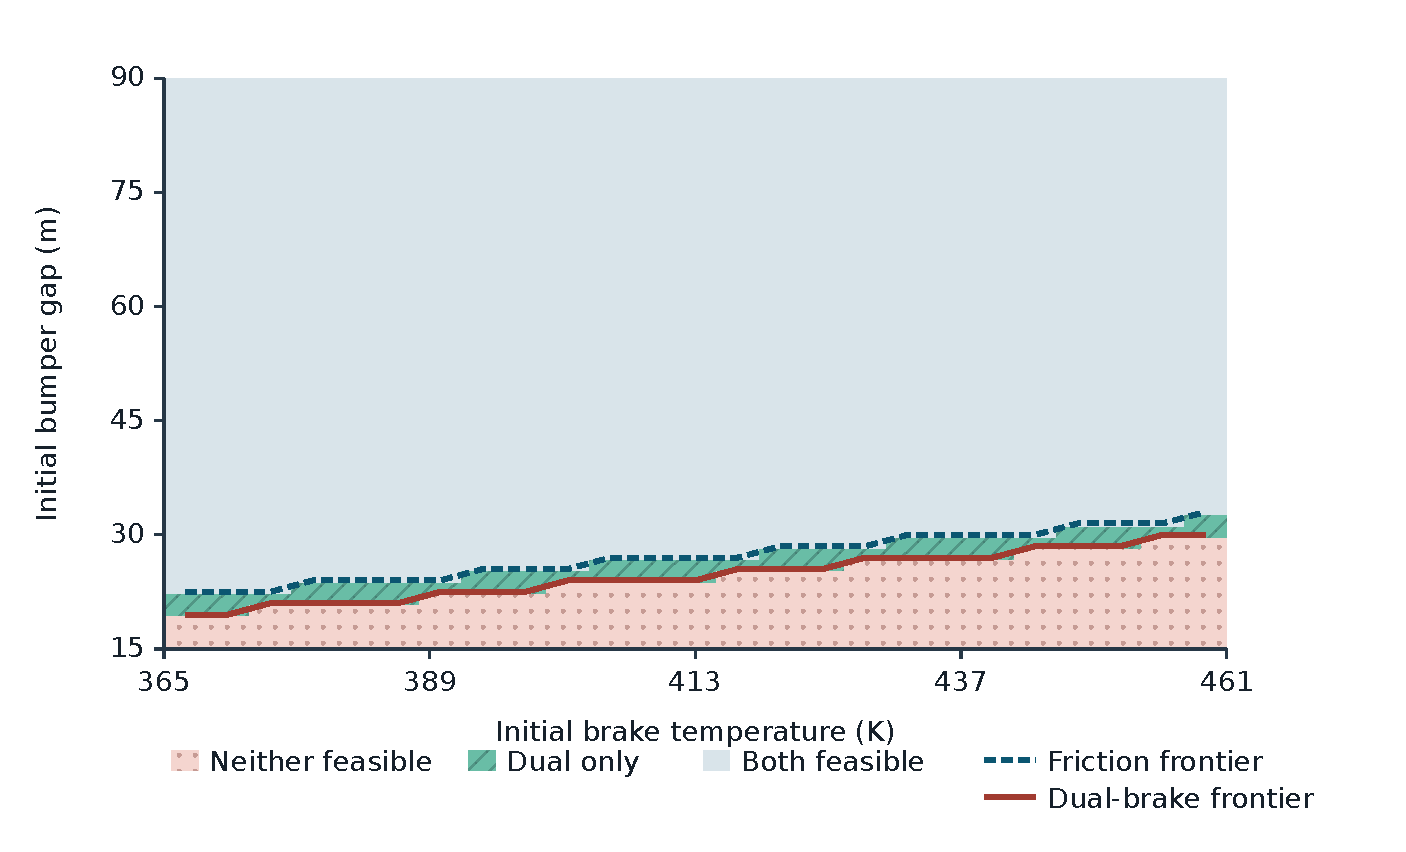
\includegraphics[width=.9\textwidth]{../generated/submission_revision/figures/feasibility_frontier.pdf}
\caption{Initial-command feasibility in the separate 1,275-state boundary follow-up at 15~m/s on a 10\% downgrade. Color and pattern classify the hard set by temperature and gap; dashed/solid curves are friction-only/dual-brake zero-reserve boundaries. The green band is dual-only feasible.}
\label{fig:feasibility-frontier}
\end{figure*}

All four M2 strategies have negative minimum $\rho$ (Table~\ref{tab:phase2m-controller}), so none is universally safe. Allocation changes energy, tracking, and temperature without identifying a learning advantage. M3 loses the certificate earlier as initial temperature nears $T_{\rm crit}$ (Table~\ref{tab:final-model-evidence}).

Across three matched 100-step, three-truck ablations, both supervisors have zero certificate losses on ordinary/hot descents and six in leader braking; pairwise minima are 0.059, 0.023, and $-2.076$. Predictive/upstream triggering adds 156, 300, and 294 anticipatory truck-samples but no observed loss reduction.

\begin{table*}[!t]
\centering
\caption{Selected model-based evidence from the Phase 2M analysis.}
\label{tab:final-model-evidence}
\normalsize
\begin{tabular}{@{}lp{.35\textwidth}lp{.28\textwidth}@{}}
\toprule
Study & Quantity & Result & Interpretation \\
\midrule
M1 & Dual/friction feasible points & 270/288; 270/288 & No count increase in M1 sweep \\
M1 & Positive dual-reserve gain & 192/288 & Margin improvement only \\
M3 & Certificate loss at $T_0=413.7$ K & 16.4 s & collision\_demand \\
M3 & Certificate loss at $T_0=453.7$ K & 11 s & collision\_demand \\
M3 & Certificate loss at $T_0=461.7$ K & 10 s & collision\_demand \\
\bottomrule
\end{tabular}
\end{table*}

\begin{table*}[!t]
\centering
\caption{Matched long-descent deterministic controller comparison; method names abbreviate source-code identifiers.}
\label{tab:phase2m-controller}
\normalsize
\begin{tabular}{@{}lrrrrr@{}}
\hline
Method & Peak $T$ (K) & Min. $\rho$ & $E_f$ (MJ) & $E_a$ (MJ) & Speed RMSE (m/s) \\
\hline
Aux.-first & 458.81 & -28.532 & 12.265 & 25.978 & 2.8775 \\
Fric.-first & 458.8 & -10.141 & 13.233 & 24.796 & 2.3195 \\
Fric.-only & 364.36 & -364.1 & 1.1293 & 0 & 15.938 \\
Dual QP & 458.83 & -17.98 & 12.812 & 25.258 & 2.5585 \\
\hline
\end{tabular}
\end{table*}


\subsection{Predictive, Robustness, Communication, and Low-Speed Evidence}
M4 has no predictive or instantaneous crossing and is inconclusive. M5 verifies prefix-horizon monotonicity; longer horizons can lower numerical reserve (Table~\ref{tab:phase2m-predictive}).

\begin{table*}[!t]
\centering
\caption{Predictive-monitor metrics; dashes denote no crossing, and ``yes'' verifies M5 prefix monotonicity.}
\label{tab:phase2m-predictive}
\normalsize
\begin{tabular}{@{}lrrrrrp{.20\textwidth}@{}}
\hline
Case & Trigger (s) & Boundary (s) & Warning (s) & Vehicle & Step & Component / status \\
\hline
M4 & -- & -- & -- & 1 & 3 & friction interval \\
M5 $H=1$ & -- & -- & -- & -- & -- & yes \\
M5 $H=3$ & -- & -- & -- & -- & -- & yes \\
M5 $H=5$ & 0 & -- & -- & -- & -- & yes \\
M5 $H=10$ & 0 & -- & -- & -- & -- & yes \\
\hline
\end{tabular}
\end{table*}


Among \FollowupScenarioCount{} boundary approaches are \FollowupTrueWarningCount{} isolated early warnings, \FollowupConservativeWarningCount{} nonisolated warnings, and \FollowupSimultaneousWarningCount{} simultaneous crossings; only \FollowupRobustTrueWarningCount{} satisfy the strict adjacent-grid/finite-margin rule (Fig.~\ref{fig:predictive-examples}). At all 32,849 stored numerically positive predictive vehicle-samples, concurrent $\rho_i\ge0$ (minimum 0). This checks implementation consistency, not sound enclosure: the tube check samples 5,000 states, and negative predictions remain inconclusive warnings.

\begin{figure*}[t]
\centering
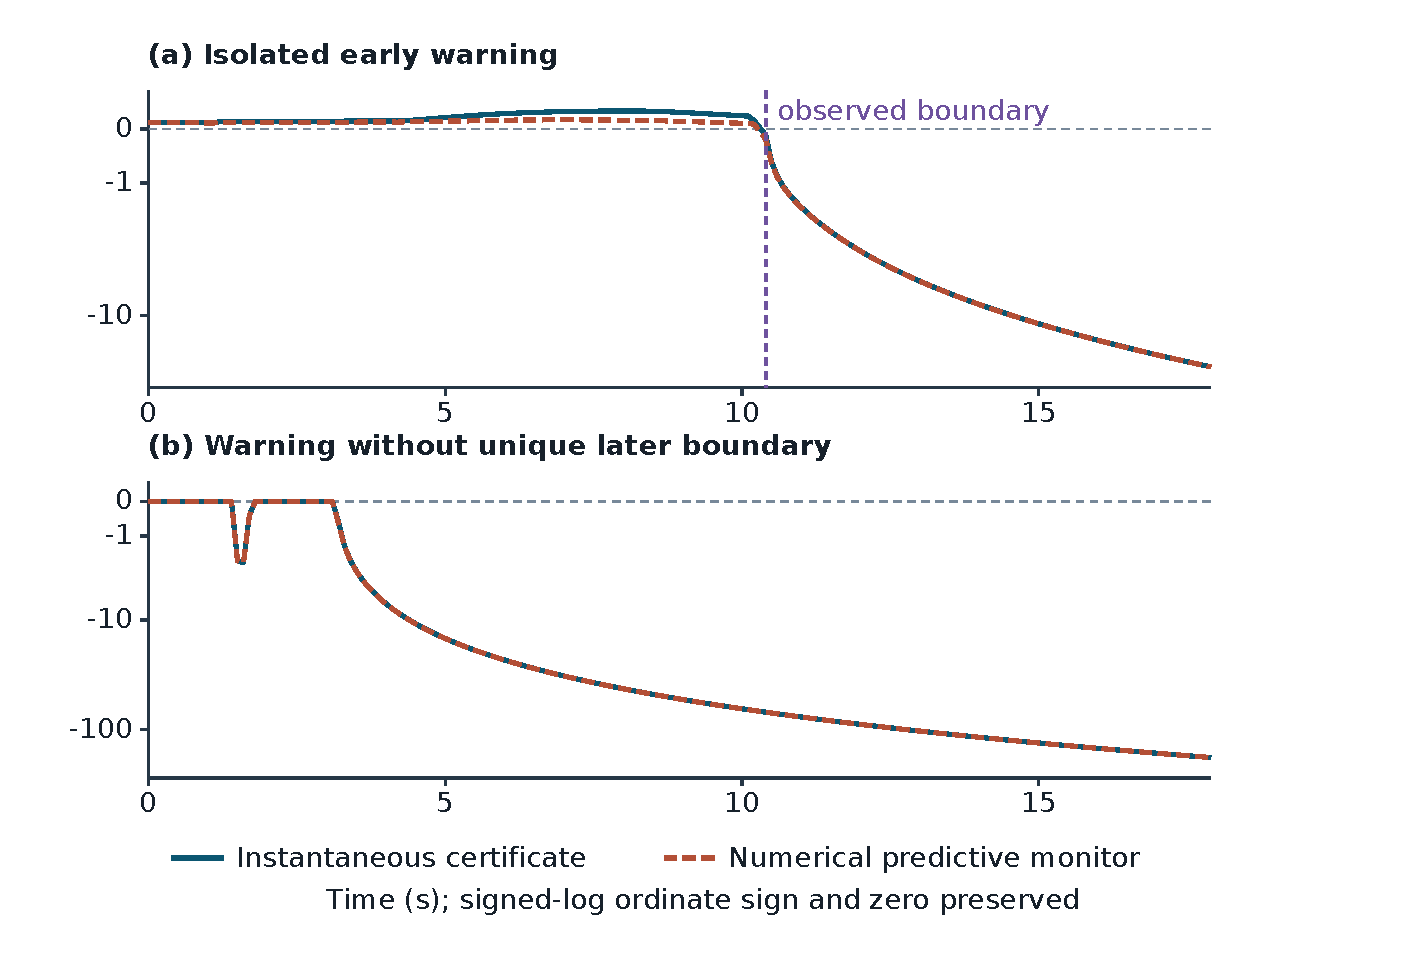
\includegraphics[width=.9\textwidth]{../generated/submission_revision/figures/predictive_examples.pdf}
\caption{Follower-1 instantaneous certificate $\rho_i$ and numerical predictive monitor $\widehat{\rho}_{i,k}^{H}$: isolated early warning (top) and nonisolated warning (bottom). Signed-log scaling preserves zero; these model-based traces are not verified reachable-set bounds.}
\label{fig:predictive-examples}
\end{figure*}

M6 includes one endpoint certificate loss and losses in 3/20 joint design samples. These deterministic samples are not a physical probability law or reliability estimate; complete rows are archived.

A 300-point stratified design varies bounded mass, friction lag, cooling, force limit, auxiliary capacity, and fade-temperature offset near 413~K/24~m. It yields 133 nonnegative initial reserves (range $-1.505$ to 0.059); collision demand limits 172 points and the auxiliary interval 128. These are sensitivity, not failure-probability, results. Zero-width declared intervals fix thermal capacity and auxiliary lag.

M7 shows stale fleet awareness: head-truck mean absolute error against the centralized oracle rises from $3.1\times10^{-6}$ at zero delay to 0.027, 0.055, and 0.078 at 100, 200, and 300~ms. Nominal 50/100~ms delays coincide under 100-ms sampled consumption. Critical-vehicle agreement falls from 1.00 to 0.62, 0.64, 0.62; missed/false triggers are 9/8, 7/10, 6/11, not monotone despite rising mean error. Bounded-delay and stale-message cases each reach 1.118 mean head gap and 112 false triggers (Fig.~\ref{fig:communication}). Non-head vehicles aggregate only their upstream subchain, lowering vehicle-level agreement even at zero delay.

\begin{figure*}[t]
\centering
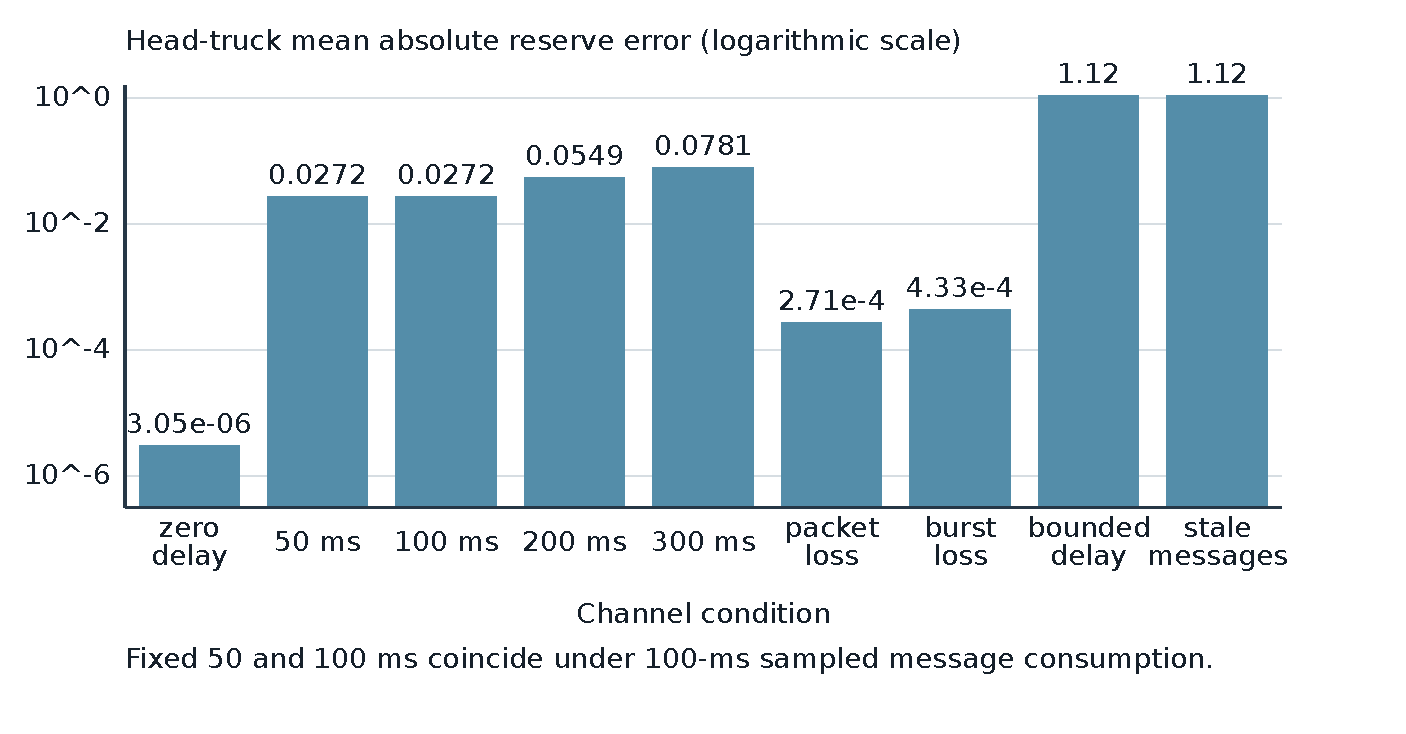
\includegraphics[width=.9\textwidth]{../generated/submission_revision/figures/communication_age.pdf}
\caption{Head-truck age-aware reserve error against the instantaneous oracle under delay/loss/staleness (log scale; 120 samples per case). The 50/100-ms cases coincide under 100-ms sampled consumption.}
\label{fig:communication}
\end{figure*}

M8 rows remain finite but the hot-brake reserve jumps at $v_\epsilon$: ZOH and high-order barrier branches are distinct sufficient conditions, so normalized reserves need not match. Smoothing would compromise exact feasibility; the hard switch remains, without implying physical discontinuity. The supervisor reverifies changed commands. M9 fails the preregistered numerical string-stability criterion in grade transitions; no such theorem is claimed.

M10 measures computation only on the recorded Windows/Python test platform. The worst tested 99th-percentile controller time (P99) is below the 100-ms sampling period; component-wise measurements remain in the source package. This is neither target-hardware certification nor a real-time guarantee.

\subsection{Formal Learning and Conditional Differentiation}
Regular-case tests validate the local KKT derivative, but paired learning encounters nonregular QP sets on every tested sample: gradient-valid fraction \FinalGradientValid{}, fallback \FinalFallback{}. DiffQP and matched StopGradient have identical recorded returns/interventions, without evidence of a learning advantage. Forward projection is unchanged; ten-seed details are archived.

\subsection{Adapted External-Baseline Comparison}
All six matched transfer pairs have zero geometric collisions. Peak brake temperature is lower in each proposed-method case (362.43--461.71~K versus 479.24--658.92~K for adapted Zhou \emph{et al.}); fade-envelope violations are zero versus 1,139 total. This exposes a constraint absent from the fixed scalar-acceleration adapter, not native-algorithm superiority. Per-case rows and adapter code accompany the source.

The post-hoc numerical counterpart $\widehat{\rho}^{H}$ is negative for the adapted baseline in all six cases; the proposed predictor is negative in four and nonnegative in two. Neither unconditional feasibility nor universal predictive superiority follows.

Speed/spacing root-mean-square errors and jerk RMS are lower in all six proposed-method pairs; auxiliary energy is higher in five, friction energy lower in six. These deterministic results do not imply general learning or efficiency gains. The adapted baseline is faster on the measured platform: P99 0.232--0.328~ms versus 1.037--1.522~ms. The proposed stack includes thermal/fade rows, tube, bottleneck, and supervision; neither timing is target-hardware certification.

Scalar-acceleration adaptation to two brake commands, observation mapping, no heavy-duty retraining, and prespecified unreported source details limit this domain-transfer stress test; it is no native-domain ranking.

\section{Discussion and Limitations}
The certificate attributes vehicle-physical conflict: heating contracts friction authority; auxiliary braking can restore it only within gear, speed, power, and lag limits. The dual-only frontier and matched ablation distinguish \emph{available authority} from \emph{realized benefit}. Positive normalizer changes preserve certificate signs but can change attribution: across 288 M1 states, multiplying one of $s_f,s_a,s_M$ by 0.5 or 2 preserves every sign, with component agreement 0.896--1.000. Trigger-time sensitivity was not measured.

Communication age changes recursive reserve and attribution; the zero-delay head minimum matches the centralized oracle. The nominal controller can vary. Finite-horizon theory still requires sound uncertainty/reserve enclosures and final-action reverification; the floating-point predictor is unverified. The numerical low-speed certificate retains its hard branch switch, without unsafe interpolation.

The literature-calibrated composite is not an identified truck; its lumped thermal model omits wheel-end imbalance/spatial gradients. There is no field or hardware-in-the-loop validation, string-stability theorem, or universal closed-loop feasibility claim. Active-set degeneracy disables QP-mediated learning gradients in the formal campaign; external transfer is adapter-sensitive and timing platform-specific. Vehicle identification and communication-aware validation remain necessary.

\section{Conclusion}
A vehicle-level dual-brake feasibility problem was formulated for heavy-duty platoons under collision demand, friction heating/fade, and auxiliary-actuator limits. Its two-command instantaneous certificate exactly tests nonemptiness of the declared hard set, independently of the nominal controller. A theoretical one-sided finite-horizon extension requires sound enclosure; the evaluated floating-point predictor remains a numerical monitor. An age-aware V2V bottleneck informs four-mode supervision and final-command reverification. Of 1,275 targeted initial states, 43 are dual-only feasible; matched same-plant runs show no certificate-loss reduction in three tested cases, while communication delay degrades upstream awareness. Vehicle-specific identification, verified interval implementation, hardware-in-the-loop tests, heavy-truck experiments, and embedded timing validation are needed before operational use.

\appendices
\section{Expanded Affine Rows and Checks}
For linear $\alpha_{1c}(s)=k_{1c}s$ and $\alpha_{2c}(s)=k_{2c}s$, substitution of \eqref{eq:jerk} into \eqref{eq:hcddot} gives the collision row coefficients in \eqref{eq:collision_hocbf} and the nominal uncontrolled term
\begin{align}
\widehat\Xi_i^c={}&a_{i-1}-a_i-\frac{a_i^2}{a_i^S}
-c_i\!\left(\frac{\widehat{\dot F_i^r}}{m_i}+\frac{b_i}{m_i\tau_i^f}+\frac{r_i}{m_i\tau_i^a}\right)\nonumber\\
&+\frac{a_{i-1}^2}{a_{i-1}^E}+r_{i-1}^v\widehat{\dot a}_{i-1}
+(k_{1c}+k_{2c})\dot h_i^c+k_{1c}k_{2c}h_i^c.
\end{align}
Thus the signs of both command coefficients are positive. The thermal expansion follows directly from
\begin{equation}
\ddot h_i^T=-\frac{\eta_i}{C_i}(\dot b_iv_i+b_ia_i)
+\frac{k_i}{C_i}(\dot T_i-\dot T_a)-\frac{\dot q_i^w}{C_i},
\end{equation}
and $\dot b_i=(-b_i+u_i^f)/\tau_i^f$, which gives the negative friction-command coefficient in \eqref{eq:thermal_hocbf}. For fade,
\begin{equation}
\dot h_i^F=\bar b_i\phi_i'(T_i)\dot T_i+\frac{b_i-u_i^f}{\tau_i^f},
\end{equation}
whose rearrangement is exactly \eqref{eq:fade_cbf}.

For the auxiliary envelope, $\dot h_i^A=\bar r_{i,v}a_i+(r_i-u_i^a)/\tau_i^a$; rearranging $\dot h_i^A+\alpha_A(h_i^A)\ge\gamma_i^A+\mu_i^A$ gives \eqref{eq:auxcbf}. For the low-speed row, variation of constants applied to the cascaded first-order friction actuator and thermal state produces the kernels $I_{0i}$ and $I_{1i}$ in \eqref{eq:zohthermal}. Since $I_{0i}-I_{1i}\ge0$, the row is an upper bound on $u_i^f$ for $v_i>0$ and degenerates continuously to $0\le g_{i,k}^{T0}$ at $v_i=0$. The latter term is retained independently in \eqref{eq:rho}, so a negative state-only reserve cannot be hidden by nonempty command intervals.

Jerk is a post-action comfort outcome, not a QP row, slack, or coordinate. Symbolic checks verify the collision, thermal, fade, and auxiliary rows. Equation regression uses 10,000 physical cases in each of five families: collision and thermal differentiation/affine/QP agreement, fade rearrangement, auxiliary-envelope rearrangement, and exact-reserve agreement. Hot/cold low-speed tests cover $v=0$, $v\approx0$, $v=v_\epsilon$, and $v>v_\epsilon$, including the exclusive HOCBF/ZOH partition and state-only infeasibility when $g^{T0}<0$. Predictive checks use 10,000 independent interval-box LP vertex solves, the zero-uncertainty $H=1$ reduction, 5,000 sampled tube states, and fleet min/argmin and trigger tests. These are regression checks, not proofs of identified uncertainty bounds, continuous-time containment, arbitrary state-feedback monotonicity, or field safety.


\bibliographystyle{IEEEtran}
\bibliography{references}
\end{document}
